\documentclass[tikz, margin=2]{standalone}
\usepackage{amsmath}


\begin{document}
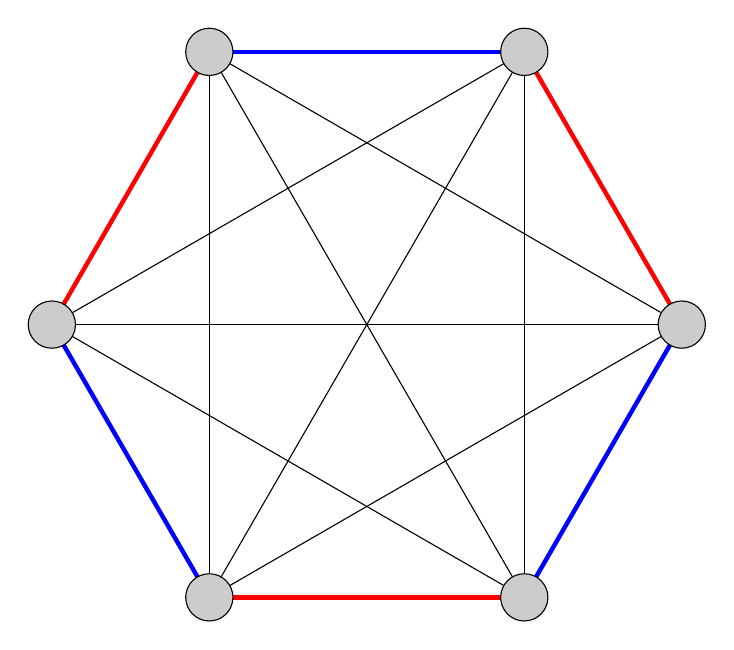
\begin{tikzpicture}

% Draw the rim in color
\draw[color=red,ultra thick] (0,0) -- (4,0);
\draw[color=red,ultra thick] (-2,3.464) -- (0,6.928);
\draw[color=red,ultra thick] (4,6.928) -- (6,3.464);
\draw[color=blue,ultra thick] (0,0) -- (-2,3.464);
\draw[color=blue,ultra thick] (0,6.928) -- (4,6.928);
\draw[color=blue,ultra thick] (6,3.464) -- (4,0);

% Draw all the other edges
\draw (0,0) -- (0,6.928);
\draw (0,0) -- (4,6.928);
\draw (0,0) -- (6,3.464);
\draw (-2,3.464) -- (4,6.928);
\draw (-2,3.464) -- (6,3.464);
\draw (-2,3.464) -- (4,0);
\draw (0,6.928) -- (6,3.464);
\draw (0,6.928) -- (4,0);
\draw (4,6.928) -- (4,0);

% Draw the nodes
\filldraw[color=black,fill=gray!40] (0,0) circle (.3);
\filldraw[color=black,fill=gray!40] (-2,3.464) circle (.3);
\filldraw[color=black,fill=gray!40] (0,6.928) circle (.3);
\filldraw[color=black,fill=gray!40] (4,6.928) circle (.3);
\filldraw[color=black,fill=gray!40] (6,3.464) circle (.3);
\filldraw[color=black,fill=gray!40] (4,0) circle (.3);

\end{tikzpicture}
\end{document}
